\newpage
	\section{Листок 2}
		\subsection*{Задача 1}
		\textbf{Условие}\\
		Пусть $X = \left[0, 1\right)\cup \left[2, 3\right)\cup\{4\}$ (с топологией, индуцированной из $\mathbb{R}$). Существует ли подмножество $Y\subset \mathbb{R}$, которому гомеоморфна одноточечная компактификация $X_{+}$ пространства $X$? Существует ли локально компактное пространство, не гомеоморфное $X$, одноточечная компактификация которого гомеоморфна $X_{+}$?\\
		\\
		\textbf{Решение}\\
		Рассмотрим $Y = [0,2] \cup \{4\}$\\
		Отображение $f:\ X_{+} \to Y$\\
		\begin{gather*}
			f(x) = 
			\begin{cases}
				x:\quad  x \in \left[0,1\right) \cap \{4\}\\
				4 - x:\quad  x \in \left[2,3\right)\\
				1:\quad  x = \infty
			\end{cases}
		\end{gather*}
		\begin{comment}
		f^{-1}(x) = 
		\begin{cases}
		x:\quad  x \in \left[0,1\right) \cap \{4\}\\
		4 - x:\quad  x \in \left(1,2\right]\\
		\infty:\quad  x = 1
		\end{cases}
		\end{comment}	
		Для любого открытого $U \subset Y,\ 1 \notin U:\quad f^{-1}(U)$ -- соотв. открыто в $X\ \Rightarrow$ открыто в $X_{+}$\\
		Рассмотрим $U \subset Y\quad f^{-1}(U) = (\alpha, 1) \cup (4-\beta, 3) \cup \{\infty\}$ где $\alpha \in \left[0,1\right),\ \beta\in \left(1,2\right],\ 1\in (\alpha, \beta) = U$\\
		Тогда $X_{+}\slash f^{-1}(U) = X\slash f^{-1}(U) = [0, \alpha] \cup [\beta, 2] \cup \{4\}$ -- ограничен и замкнут $\Rightarrow$ компакт $\Leftrightarrow$ $f^{-1}(U)$ открыто в топологии $X_{+}$\\
		Обратно аналогично $\Rightarrow$ $f$ -- гомеоморфизм\\
		\\
		Локально компактное пространство $Z \simeq X,\ Z_{+} \simeq X_{+}$, $Z = \left[0,1\right) \cup \{4\}$ или $Z = [0,1]$\\	
		\\\\
		
		\begin{comment}
		
		
		$x = \left[0,1\right) \cup \left[2,3\right) \cup \{4\}$\\
		$x^{\prime} = \left[0,1\right) \cup \left(1,2\right] \cup \{4\}$\\
		\\
		Докажем, что $x \simeq x^{\prime}$:
		\begin{gather*}
		f(x) = 
		\begin{cases}
		x,\quad x \in \left[0,1\right) \cup \{4\}\\
		1 + (3 - x),\quad x \in \left[2,3\right)
		\end{cases}\\
		f^{-1}(x) = 
		\begin{cases}
		x,\quad x \in \left[0,1\right) \cup \{4\}\\
		x-4,\quad x \in \left(1,2\right]
		\end{cases}
		\end{gather*}
		Рассмотрим множества, открытые в $x^{\prime}$, это
		\begin{enumerate}
		\item $(a,b)$
		\item $\left[0,a\right),\quad a \leqslant 1$
		\item $\left(a,2\right],\quad a \geqslant 1$
		\item $\{4\}$
		\end{enumerate}
		Рассмотрим множества, открытые в $x$, это
		\begin{enumerate}
		\item $(a,b)$
		\item $\left[0,a\right),\quad a \leqslant 1$
		\item $\left[2,a\right),\quad a \leqslant 3$
		\item $\{4\}$
		\end{enumerate}
		Прообраз открытого открыт
		\begin{gather*}
		\left[a,b\right) \to \left[a,b\right)\\
		\left[0,a\right) \to \left[0,a\right)\\
		\left[2,4-a\right) \to \left[2,a\right)\\
		\{4\} \to \{4\}
		\end{gather*}
		откуда следует что функция непрерывна\\
		\\
		Заметим что $[0,2] \cup \{4\}$ является одноточечной компактификацией $\left[0,1\right) \cup \left(1,2\right] \cup \{4\}$, так как 
		Рассмотрим ${x^{cprime}}_{+} = \left[0,2\right] \cup \{4\}$\\
		Если два пространства гомеоморфны, то и соответственные компактификации гомеоморфны: $x \cong x^{\prime}\ \Rightarrow {x}_{+} \cong {x^{\prime}}_{+}$, откуда $y = {x^{\prime}}_{+}$\\
		\\
		Рассмотрим $A = \left[0,2\right) \cup \{4\}$ -- локально компактно\\
		В $A$ существуют 2 компоненты связности, в $x$ -- три\\
		Откуда $A \not\cong x$, ${A}_{+} = x_{+} = \left[0,2\right] \cup \{4\}$, откуда $A_{+} \cong x_{+}$, откуда следует, что $A$ -- искомое множество\\
		\end{comment}
		
		\subsection*{Задача 2}
		\textbf{Условие}\\
		Постройте гомеоморфизм между $[0,1] /\left[\frac{1}{3}, \frac{2}{3}\right]$ и $[0,1]$\\
		\\
		\textbf{Решение}\\
		Универсальное свойство факторпространств: $Y$ -- топологическое протранство, $f: X \to Y$ -- непрерывное отображение, построенное на классах эквивалентности, то есть $x \sim y\ \Rightarrow\ f(x) = f(y)$\\
		Тогда $\exists!$ непрерывное отображение $\tilde{f}$, делающее эту диаграмму коммутативной\\
		\begin{wrapfigure}{h}{0.2\textwidth}
			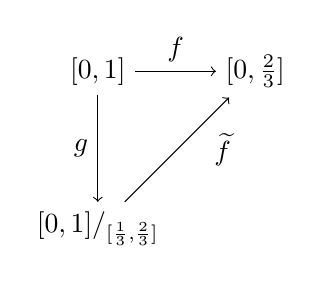
\begin{tikzpicture}[node distance=2cm, auto]
				\node (X) {$[0,1]$};
				\node(Y) [right of=X] {$[0, \frac{2}{3}]$};
				\node (X1) [below of=X] {$[0,1]\slash_{[\frac{1}{3},\frac{2}{3}]}$};
				\draw[->](X) to node [left]{$g$}(X1);
				\draw[->](X1) to node [right]{$\quad \widetilde{f}$}(Y);
				\draw[->](X) to node {$f$}(Y);
			\end{tikzpicture}
		\end{wrapfigure}
		\begin{gather*}
			f(x) = 
			\begin{cases}
				x,\quad x \in \left[0, \frac{1}{3}\right)\\
				\frac{1}{3},\quad x \in \left[\frac{1}{3}, \frac{2}{3}\right]\\
				x-\frac{1}{3},\quad x \in \left(\frac{2}{3}, 1\right]
			\end{cases}
		\end{gather*}
		$\Rightarrow \exists! \tilde{f}$ непрерывна: $x \sim y\ \Rightarrow$ одноэлементные $\to$ одноэлементные, $[\frac{1}{3}, \frac{2}{3}]$ склеивается в 1 точку(*)\\
		Универсальное свойство выполняется. Тогда известно, что:
		\begin{enumerate}
			\item $\tilde{f}$ -- сюръекция $\Leftrightarrow\ f$ -- сюръекция
			\item $\tilde{f}$ -- инъекция $\Leftrightarrow\ \forall x,y \in X\quad x \sim y \Leftrightarrow f(x) = f(y)$ (показано ранее в (*) $\Rightarrow$ инъекция) 
		\end{enumerate}
	 	$f$ -- сюръекция:\\
	 	$\forall x \in \left[0, \frac{1}{3}\right)\quad f(x) = x$ -- на $\left[0, \frac{1}{3}\right)$ сюръекция,\\
	 	$x = \frac{1}{3}:\quad f([\frac{1}{3}, \frac{2}{3}]) = \frac{1}{3}$ -- $\{\frac{1}{3}\}$ сюръекция,\\
	 	$\forall x\in \left(\frac{1}{3}, \frac{2}{3}\right]:\quad f(x + \frac{1}{3}) = x$ --  $\left(\frac{1}{3}, \frac{2}{3}\right]$ сюръекция\\
		Откуда следует что $f$ -- сюръекция $\Rightarrow\ \tilde{f}$ -- сюръекция\\
		То есть $\tilde{f}$ -- инъекция и сюръекция\\
		Если $[0,1]$ компактно(а это так, так как это отрезок), а $[0, \frac{2}{3}]$ хаусдорфово, то $\tilde{f}$ -- гомеоморфизм\\
		$[0, \frac{2}{3}]$ хаусдорфово, так как 
		\begin{enumerate}
			\item 
			для $a,b:\ a<b,\ a\ne 0,\ b \ne \frac{2}{3},\ \varepsilon = b - a$ искомые окрестности: $(0, a + \frac{\varepsilon}{2}), (b - \frac{\varepsilon}{2}, \frac{2}{3})$
			\item 
			для $a,b:\ a<b,\ b \ne \frac{2}{3},\ a = 0:\ \left[0, \frac{\varepsilon}{2}\right), (\frac{\varepsilon}{2}, b)$
			\item 
			для $a,b:\ a<b,\ a\ne 0,\ b = \frac{2}{3},\ \varepsilon = b - a:\ (0, a + \frac{\varepsilon}{2}), (b - \frac{\varepsilon}{2}), \left(b - \frac{\varepsilon}{2}\right]$
			\item 
			для $a,b:\ a = 0,\ b = \frac{2}{3}:\ \left[0, \frac{1}{6}\right), \left(\frac{1}{2}, \frac{2}{3}\right)$
		\end{enumerate}
		Откуда $\tilde{f}$ -- гомеоморфизм\\
		\\
		$[0, \frac{2}{3}] \simeq [0,1]:\ x \to \frac{3}{2}x$ -- непрерывно, $f^{-1}(x) = \frac{2}{3}$ следовательно это биекция, откуда $[0,1] /\left[\frac{1}{3}, \frac{2}{3}\right]$ и $[0,1]$, что и требовалось доказать\\
		\\
		
		\begin{comment}
		\begin{gather*}
		[0,1]\slash_{[\frac{1}{3}, \frac{2}{3}]} \to [0, \frac{2}{3}] \to [0,1]\\
		f(x) = 
		\begin{cases}
		x,\quad x \in \left[0, \frac{1}{3}\right)\\
		\frac{1}{3},\quad x \in \left[\frac{1}{3}, \frac{2}{3}\right]\\
		x-\frac{1}{3},\quad x \in \left(\frac{2}{3}, 1\right]
		\end{cases}
		\end{gather*}
		$f$ непрерывна, инъективна, сюръективна\\
		$f(x)$ непрерывна на каждом куске, в каждой точке границы есть предел слева и справа $\Rightarrow$ можно выбрать минимум из двух, откуда следует, что функция непрерывна везде
		\begin{gather*}
		\forall x \in \left[ 0, \frac{1}{3} \right)\quad f([x]) = f(x) = x = [x]\\
		\forall x = \frac{1}{3}\quad f([\frac{1}{3}]) = f([\frac{1}{3}, \frac{2}{3}]) = \frac{1}{3}\\
		\forall x \in \left( \frac{1}{3}, \frac{2}{3} \right]\quad f([x]) = f(x) = x = [x]
		\end{gather*}
		$f$ -- сюръективна, так как
		\begin{gather*}
		\forall x \in \left[ 0, \frac{1}{3} \right)\quad f(x) = x = [x]\\
		\forall x = \frac{1}{3}\quad f([\frac{1}{3}, \frac{2}{3}]) = x\\
		\forall x \in \left(\frac{1}{3}, \frac{2}{3} \right]\quad f(x + \frac{1}{3}) = x
		\end{gather*}
		$f^{-1}$ тоже непрерывна\\
		Откуда следует, что $f$ гомеоморфизм\\
		$g: [0, \frac{2}{3}] \to [0,1]\quad g(y) = \frac{3}{2}y$ -- гомеоморфизм\\
		композиция гомеомрфизмов также гомеоморфизм\\
		\begin{gather*}
		\tilde{f}(x) = g \circ f(x) = 
		\begin{cases}
		\frac{3}{2}x,\quad x \in \left[0, \frac{1}{3}\right)\\
		\frac{1}{2},\quad x \in \left[\frac{1}{3}, \frac{2}{3}\right]\\
		\frac{3}{2}x - \frac{1}{2},\quad x \in \left(\frac{2}{3}, 1\right]
		\end{cases}
		\end{gather*}	
		\end{comment}
		
		\begin{comment}
		$[0,1]\slash [\frac{1}{3}, \frac{2}{3}] \cong [0, \frac{2}{3}]$\\
		\begin{gather*}
		f(x) = 
		\begin{cases}
		x,\quad x \in \left[0, \frac{1}{3}\right)\\
		\frac{1}{3},\quad x \in \left[\frac{1}{3}, \frac{2}{3}\right]\\
		x-\frac{1}{3},\quad x \in \left(\frac{2}{3}, 1\right]
		\end{cases}
		\end{gather*}
		$f(x)$ непрерывна на каждом куске, в каждой точке границы есть предел слева и справа $\Rightarrow$ можно выбрать минимум из двух, откуда следует, что функция непрерывна везде
		\begin{gather*}
		\forall x \in \left[ 0, \frac{1}{3} \right)\quad f([x]) = f(x) = x = [x]\\
		\forall x = \frac{1}{3}\quad f([\frac{1}{3}]) = f([\frac{1}{3}, \frac{2}{3}]) = \frac{1}{3}\\
		\forall x \in \left( \frac{1}{3}, \frac{2}{3} \right]\quad f([x]) = f(x) = x = [x]
		\end{gather*}
		
		\begin{wrapfigure}{R}{0.2\textwidth}
		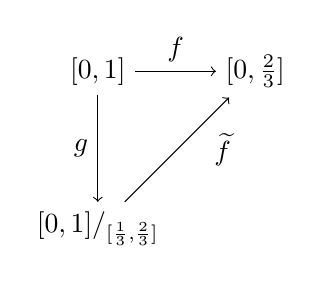
\begin{tikzpicture}[node distance=2cm, auto]
		\node (X) {$[0,1]$};
		\node(Y) [right of=X] {$[0, \frac{2}{3}]$};
		\node (X1) [below of=X] {$[0,1]\slash_{[\frac{1}{3},\frac{2}{3}]}$};
		\draw[->](X) to node [left]{$g$}(X1);
		\draw[->](X1) to node [right]{$\quad \widetilde{f}$}(Y);
		\draw[->](X) to node {$f$}(Y);
		\end{tikzpicture}
		\end{wrapfigure}
		
		$f$ -- сюръективна, так как
		\begin{gather*}
		\forall x \in \left[ 0, \frac{1}{3} \right)\quad f(x) = x = [x]\\
		\forall x = \frac{1}{3}\quad f([\frac{1}{3}, \frac{2}{3}]) = x\\
		\forall x \in \left(\frac{1}{3}, \frac{2}{3} \right]\quad f(x + \frac{1}{3}) = x
		\end{gather*}
		$x \sim y\quad \Leftrightarrow f(x) = f(y)$, так как одноэлементные классы эквивалентности переходят в себя, а не одноэлементные все склеиваются в одну точку\\
		$g: [0, \frac{2}{3}] \to [0,1]$\\
		$g(x) = \frac{3}{2}x$\\
		$g$ -- нерерывна
		$g^{-1}(x) = \frac{2}{3}\qquad g(g^{-1}(x)) = g((\frac{2}{3}x)) = \frac{3}{2} \cdot \frac{2}{3}x = x\ \Rightarrow$ биекция\\
		отрезок компактен и хаусдор	
		\end{comment}

			
		\subsection*{Задача 3}
		\textbf{Условие}\\
		Пусть $D=\{z \in \mathbb{C}:\ |z| \leqslant 1\}$. Введем на $D$ следующее отношение эквивалентности: $z \sim w$ тогда и только тогда, когда $z = i^{k}w$ для некоторого $k\in Z$. Докажите, что факторпространство $D/\sim$ гомеоморфно $D$.\\
		\\
		\begin{comment}
		\textbf{Решение}\\
		Построим $\varphi: D \to D$, $z \to \frac{z^4}{|z|^3},\ 0\to 0$\\
		\begin{wrapfigure}{h}{0.2\textwidth}
		\begin{tikzpicture}[node distance=2cm, auto]
		\node (X) {$D$};
		\node(Y) [right of=X] {$D$};
		\node (X1) [below of=X] {$D\slash_{\sim}$};
		\draw[->](X) to node [left]{$q$}(X1);
		\draw[->](X1) to node [right]{$\exists!\ h\text{ -- гомео}$}(Y);
		\draw[->](X) to node {$\varphi$}(Y);
		\end{tikzpicture}
		\end{wrapfigure}
		
		Покажем, что $\varphi$ -- факторно\\
		$D \supset \varphi^{-1}(U)$ -- открыто, докажем что это равносильно тому, что $D \supset U$ -- открыто\\
		$(\Leftarrow)$\\
		так как $\varphi$ непрерывно (в нуле непрерывно, так как любой открытый шар $B_r(0),\ r<1$ переходит в себя)\\
		$(\Rightarrow)$\\
		$\forall x \in \varphi^{-1}(U)$ -- откыт, есть открытая окрестность\\
		\\
		Такая окрестность перейдёт в окрестность такого же вида, но с большим углом и останется открытой $\Rightarrow$ $U$ -- открыт.\\
		При этом $|z_1| = |\frac{z^4_1}{|z_1|^3}| = |\frac{z^4_2}{|z_2|^3}| = |z_2|\ \Rightarrow\ \frac{z^4_1}{|z_1|^3} = \frac{z^4_2}{|z_2|^3}\ \Leftrightarrow\ z^4_1 = z^4_2\ \Leftrightarrow\ (z^2_1- z^2_2)(z^2_1 - i^2 z^2_2) = 0\ \Leftrightarrow\ (z_1 - z_2)(z_1 - i z_2)(z_1 - i z_2)(z_1 - i^3 z_2) = 0$\\
		Поэтому $\varphi(z_1) = \varphi(z_2)\ \Leftrightarrow\ z_1 \sim z_2$, то есть $\exists!\ h:\ D\slash_{\sim} \to D$\\
		\\
		\end{comment}
		\textbf{Решение}\\
		\begin{gather*}
			z = |z|(\cos(\alpha) + i\sin(\alpha))\\
			i = |i|(\cos(\frac{\pi}{2}) + i\sin(\frac{\pi}{2}))\\
			w = |w|(\cos(\beta) + i\sin(\beta))\\
			\\
			z_1\cdot z_2 = |z_1|\cdot|z_2|(\cos(\varphi_{z_1} + \varphi_{z_2}) + i\sin(\varphi_{z_1} + \varphi_{z_2}))\\
			|z|(\cos(\alpha) + i\sin(\alpha)) = |w|(\cos(\beta + \frac{\pi k}{2}) + i\sin(\beta + \frac{\pi k}{2}))\\
			z \sim w \text{ что то же самое, что и поворот $z$ на } \frac{\pi}{2}
		\end{gather*}
		\begin{wrapfigure}{h}{0.2\textwidth}
			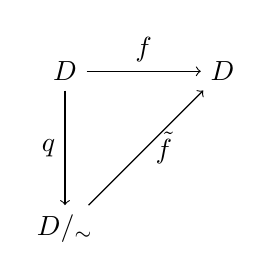
\begin{tikzpicture}[node distance=2cm, auto]
			\node (X) {$D$};
			\node(Y) [right of=X] {$D$};
			\node (X1) [below of=X] {$D\slash_{\sim}$};
			\draw[->](X) to node [left]{$q$}(X1);
			\draw[->](X1) to node [right]{$\tilde{f}$}(Y);
			\draw[->](X) to node {$f$}(Y);
			\end{tikzpicture}
		\end{wrapfigure}
		\begin{gather*}
			f: D \to D\\
			f(z) = z^4\\
			z \sim w\ \Rightarrow f(z) = f(w) \text{непрерывно на классах эквивалентности}
		\end{gather*}
		$\exists!$ отображение $\tilde{f}\ |\ \tilde{f}\circ g = f$ (из теоремы)\\
		Докажем несколько фактов:\\
		\begin{enumerate}
			\item 
				$f$ -- сюръекция, так как $\forall c \in D\quad f^{-1} = |c|^{\frac{1}{4}}(\cos(\frac{\alpha + 2\pi k}{4}) + i\sin(\frac{\alpha + 2\pi k}{4})) = |c|^{\frac{1}{4}}(\cos(\frac{\alpha}{4} + \frac{\pi k}{2}) + i\sin(\frac{\alpha}{4} + \frac{\pi k}{2}))$\\
				$c = |c|(\cos(\alpha) + i\sin(\alpha))$\\
				$\cos(\alpha) \in [-1,1]\qquad \sin(\alpha) \in [-1,1]\qquad \cos(\frac{\alpha}{4} + \frac{\pi k}{2}) \in [-1,1]\qquad \sin(\frac{\alpha}{4} + \frac{\pi k}{4}) \in [-1,1]$\\
				$\tilde{f}(D\slash_{\sim}) = \tilde{f}(q(x)) = f(x)$, откуда $\tilde{f}$ -- сюръекция
			\item
				$\forall x,y \in D\quad x \sim y$ и $f(x) = f(y)$ (условия эквивалентны)\\
				так как при $x \not\sim z$\\
				$|x|(\cos(\alpha) + i\sin(\alpha)) \ne |z|(\cos(\beta + \frac{\pi k}{2}) + i\sin(\beta + \frac{\pi k}{2}))\quad \Rightarrow \quad |x|^{4}(\cos(\varphi\alpha) + i\sin(\varphi\alpha)) \ne |z|^{4}(\cos(\varphi\beta) + i\sin(\phi\beta) + i\sin(\varphi\beta))\qquad f(x) \ne f(z)$\\
				Откуда следует что: \\
				$\tilde(f)$ -- инъекция(каждый класс эквивалентности перешел в разные элементы) \\
				$\tilde(f)$ -- непрерывная биекция
			\item
				$D$ -- компактно (так как замкнуто и ограничено в метрическом пространстве) и хаусдорфово (так как у $x_0 \ne y_0\quad \exists$ непересекающиеся окрестности: $|x - x_0| < r_1,\quad |y - y_0| < r_2$)
		\end{enumerate}
		Откуда следует что $\tilde{f}$ -- гомеоморфизм\\
		\\
		
		\subsection*{Задача 4}
		\textbf{Условие}\\
		Пусть $X$ -- подмножество в произведении $\{0, 1\}^S$ несчетного семейства двоеточий $\{0, 1\}$, состоящее из всех тех элементов, у которых не более чем счетное число координат отличны от нуля. (Пространство $\{0, 1\}$ здесь снабжается дискретной топологией, а пространство $\{0, 1\}^S$ -- топологией произведения, или, что то же самое, топологией поточечной сходимости.) Докажите, что $X$ секвенциально компактно, но не замкнуто в $\{0, 1\}^S$ и потому не компактно.\\
		\\
		\textbf{Решение}\\
		Для начала, попытаемся понять, что из себя представляет топология произведения или топология поточечной сходимости. База в топологии произведения -- произведение открытых множеств, на счетном числе которых стоят открытые множества из $X_i$, а на остальных - $X_j$. (тоже проверяем определение)\\		
		В нашей задаче мы можем рассмотреть такие элементы из базы, на счетном числе которых стоят $1$, на остальных -- двоеточия $\{0, 1\}$\\
		Что такое окрестность элемента $a$? Это какое-то открытое множество из базы, то есть окрестность на счетном числе координат принимает такие же значения, как и $a$, а в остальных $\{0, 1\}$.\\		
		Пусть $X$ не замкнуто. Рассмотрим дополнение к $X$ -- последовательности из несчетного числа $0$ и $1$. окрестности элементов из дополнения к $X$ могут быть такими: счетное количество $1$ и на остальных координатах $\{0, 1\}$. То есть окрестности дополнения пересекаются с $X$. Следовательно дополнение к $X$ не является открытым множеством, откуда $X$ не замкнуто.\\		
		Теперь мы докажем, что у любой последовательности есть сходящаяся подпоследовательность. Предленьная точка: cуществует номер начиная с которого все члены последовательности лежат в рассмтриваемой окрестности.\\
		
		\begin{comment}
		Рассмотрим последовательность $(Cn)$ так как $\{0,1\}$ снабжается дискретной топологией, а пр-во $\{0,1\}^S$ -- топологией поточечной сходимости, то 
		$(An)$ сходится к $b \Leftrightarrow$ $ \exists N:\ \forall n>N\ a_n=b$ (то есть координаты совпадают).\\		
		Так как каждый член последовательности принимает значение 1 не более чем в счетном числе координат, то количество координат, в которых хотя бы одна функция принимает значение 1 - тоже счетно.\\		
		Поэтому рассмотрим не более чем счетное число координат (пусть их будет $N$), в которых значение членов последовательности не $0$.\\		
		Возьмем первую координату. в ней бесконечное кол-во членов последовательности принимает значение 0, или бесконечное кол-во членов последовательности принимает значение $1$, или и то, и другое. (не может быть такого, что и тех, и тех членов последовательности конечное число, так как в таком случае у нас $(Сn)$ конечно)\\		
		Выбираем то множество членов последовательности, которое бесконечно. Находим элемент с наименьшим номером в последовательности $(Cn)$ и присваиваем ему первый номер в нужной нам подпоследовательности.\\		
		Теперь рассматриваем только выбранное нами подмножество членов последовательности. продолжая, рассматриваем оставшуюся $N-1$ координату.\\		
		У нас получилась нужная нам последовательность, которая сходится в $N$ координатах к выбранному нами элементу (1 или 0), и к 0 во всех остальных.\\		
		$X$ не замкнуто, так как не содержит все предельные точки	
		\end{comment}
		
		\subsection*{Задача 5}
		\textbf{Условие}\\
		Пусть $X$ -- произведение континуального семейства двоеточий. Заметим, что $X$ компактно в силу теоремы Тихонова. Покажите, что $X$ не является секвенциально компактным.\\
		\\
		\textbf{Решение}\\
		$X$ -- компактно и не секвенц. $X = \{0, 1\} \times \{0, 1\} \times \ldots$ компактно, Найдем последовательность у которой нет сходящейся подпоследовательности\\
		Построим биекцию между континуальным семейством двоеточий и континуумом последовательностей из 0 и 1.\\
		Построим последовательность в $X$:\\
		$a_1$ -- первая координата последовательности(которая соответствует 0 или 1), $a_2$ -- вторая координата, и так далее\\
		Тогда, выбрав последовательность, мы выбрали номера координат последовательностей, которые однозначно соответствуют $\{0,1\}$\\
		Следовательно найдется такой элемент $a_m$, что $a_m = 010101\ldots\ \Rightarrow$ подпоследовательность не сходится\\
		То есть $\forall a_i\ \exists$ набор из 0 и 1 не имеющий предела
		
		\begin{comment}
		Сопоставим каждому двоеточию некую последовательность из 0 и 1 (так мы построили биекцию с континуальным множеством)\\
		Пусть $a_i$ -- множество(континульная последовательность) $i$-ых элементов последовательностей, которые мы поставили в соответствие. Так как $X$ -- произведение континуального числа двоеточий, то и в каждом множестве(последовательности) континуум элементов, тогда там есть подпоследовательность(подмножество, являющееся последовательнотью) $0101010\ldots$, которая ни к чему не сходится(то есть не скходится ни к 0, ни к 1).
		\end{comment}
		
		\begin{comment}
		Каждое двоеточие занумеруем последовательностью нулей и единиц (так мы построили биекцию с континуальным множеством)\\
		Докажем от противного, что $X$ секвенциально компактно, тогда рассмотрим последовательность, для которой нет сходящейся подпоследовательности (существование такой последовательности следует из предположения).\\
		Заметим, что каждое двоеточие соответствует набору 0 и 1, и каждому набору 0 и 1 соответствует какое-то двоеточие(иначе это не биекция). Тогда есть элемент, выражающийся через 0 и 1 как: $0101010\ldots$, то есть бесконечная последовательность из чередующихся 0 и 1. Но у этой последовательности нет сходящейся подпоследовательности, откуда следует, что $X$ не секвенциально компактен.
		\end{comment}
		